\setchapterstyle{kao}
\setchapterpreamble[u]{\margintoc}
\chapter{Introduction}
\labch{intro}
\begin{fquote}[Douglas Adams][The Restaurant at the End of the Universe][1980] In the beginning the Universe was created. This has made a lot of people very angry and been widely regarded as a bad move. 
\end{fquote}

Multi-messenger astronomy is the youngest branch of humanity's oldest scientific discipline. Understanding the stars has long been of central importance to society, and indeed guided exploration and scientific development of the human race for many millennia. While the centrality of astronomy as a tool for navigation has long past, it continues to be a key driver of the most human of pursuits, the expansion of our understanding of the universe in which we live. 

The broad field of \emph{astroparticle physics}, particle physics with astrophysical accelerators, has been a fruitful source of mysteries in recent years. Astroparticle physics offers us the opportunity to overcome physical limitations of engineering in our quest for knowledge. While terrestrial accelerators such as the Large Hadron Collider at CERN may be capable of accelerating particles to $\sim$10 TeV, studies of cosmic rays in the past century have revealed that the universe can accelerate particles to $\sim$10 EeV, one billion times higher. Cosmic messengers can also test physics across distances of $\sim$10$^{23}$ km, rather than the $\sim$10$^{3}$ km of the Earth, and across timescales of billions of years rather than the typical decade-length horizon of research funding agencies. If we wish to study physics at these scales, competing with nature is not a viable option. Instead, we must learn to understand the dataset that nature provides for us.

\begin{figure}[!ht]
	\centering 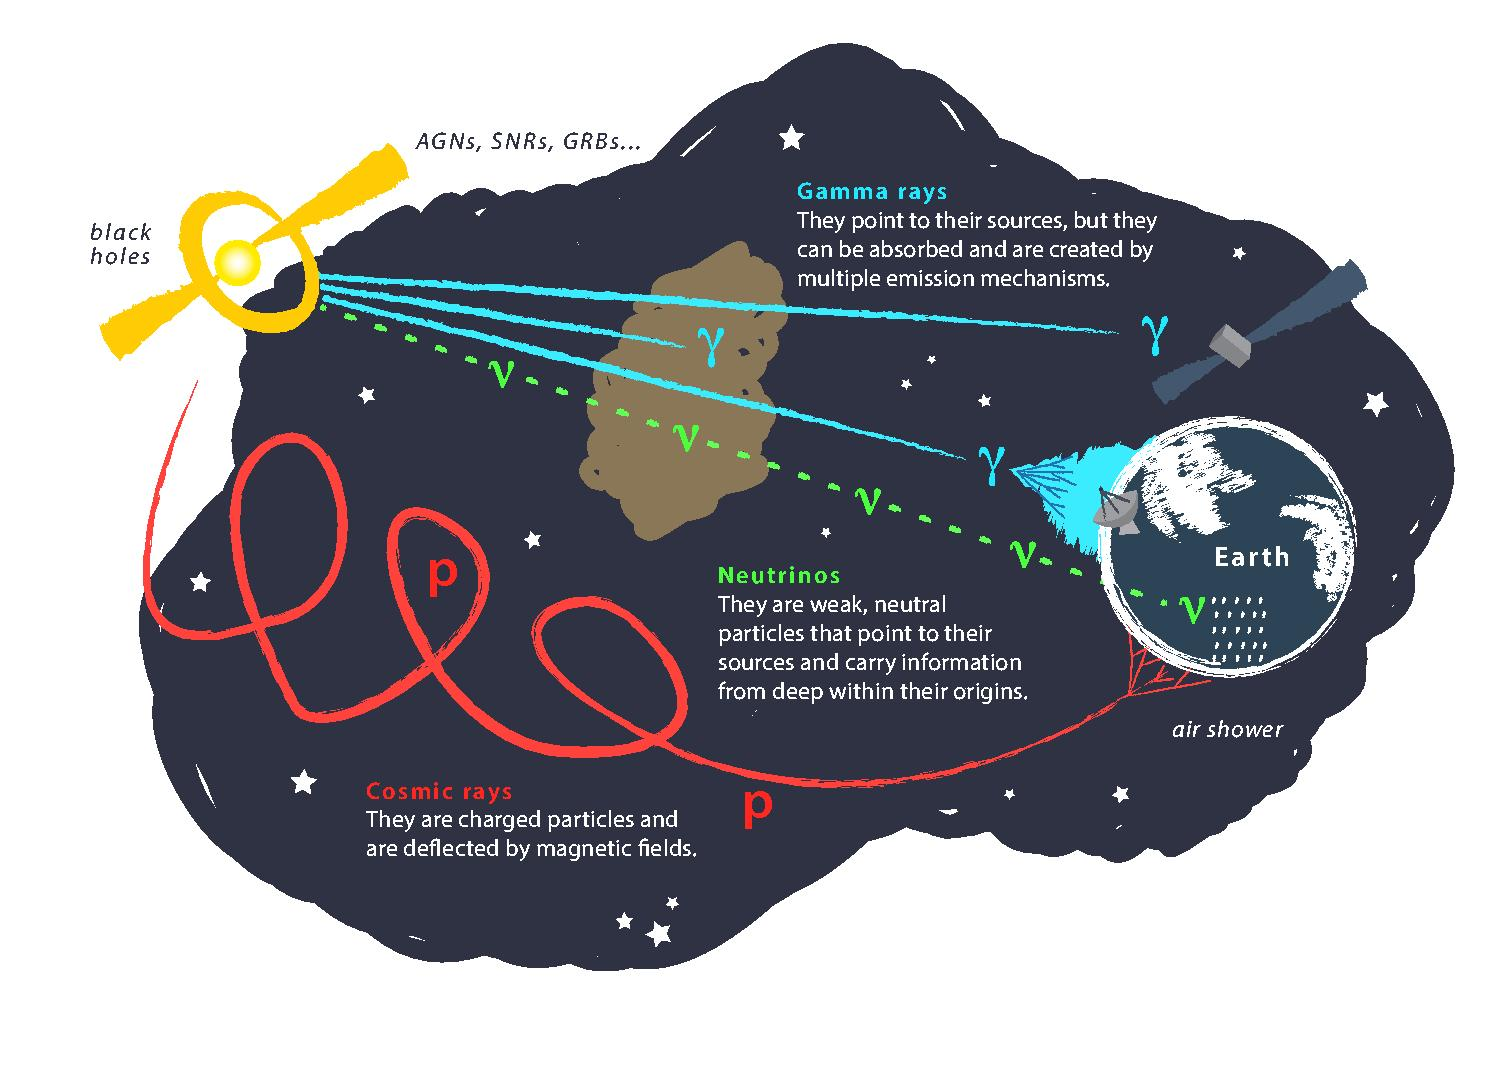
\includegraphics{mma/mm}
	\caption{An overview of multi-messenger astronomy. credit: IceCube.}
	\label{fig:mm}
\end{figure}

The existence of these high-energy charged particles \emph{cosmic rays} was first demonstrated by Victor Hess in 1912, but their origin remains unknown over a century later. In that century, the ghostly neutrino particle was first proposed by Pauli in 1930, its centrality in solar fusion was first posited by Bethe in 1939, its existence was confirmed by Cowan and Reines in 1956, the solar neutrino flux was then measured in 1964 by the Homestake with an unexpectedly-low rate (the so-called \emph{solar neutrino problem}), which then led in 2001 to the first discovery of particle physics beyond the \emph{Standard Model}, namely \emph{neutrino oscillations}. 

\begin{marginfigure}
	\centering 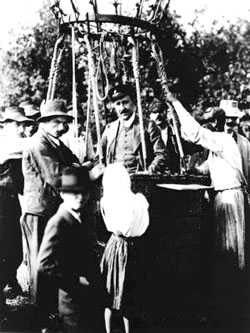
\includegraphics{intro/V-Hess-web_2.jpg}
	\caption{Victor Hess with his famous balloon, 1912. Credit?}
\end{marginfigure}

Experiments studying these solar neutrinos also accidentally provided us with the first case of observational astronomy with multiple 'messengers' (the observation of nearby supernova \emph{SN1987a} with both neutrinos and photons), followed by the discovery of extra-terrestrial high-energy \emph{astrophysical neutrinos} with the IceCube detector in 2013 produced by the very same cosmic accelerators responsible for cosmic rays. A scramble to find the origin of these neutrinos led to the birth of a new field, \emph{neutrino astronomy}. 

The long-awaited discovery of Gravitational Waves by LIGO in 2015 was shortly thereafter followed by the discovery of a Binary Neutrino Star merger, \emph{GW170817}, detected simultaneously with both photons and gravitational waves, kick-starting \emph{gravitational-wave astronomy}. One month later, the observation of a high-energy neutrino IC170922A from the direction of a flaring galactic nucleus led to the identification of the first likely source of high-energy neutrinos, \emph{TXS 0506+056}. Thirty years after \emph{SN1987a}, the year 2017 truly marked the dawn of an era of \emph{multi-messenger astronomy}. 

This thesis presents research probing the intersect of these new branches of astronomy with multiple messengers, incorporating searches for sources of neutrinos and gravitational waves using photons, and searches for photon sources using neutrinos. At its core, it seeks to understand what can be learned through combining knowledge from these new branches of astronomy with that of the oldest, namely astronomy with optical telescopes. The latter field is undergoing a revolution of its own, at the brink of transition to an algorithm-driven era dominated by enormous data volumes. Optical astronomy is moving from object-centric to population-centric science, with scales at which detailed study of individual objects is becoming infeasible. In all three fields, a focus on rapid automated responses seeks to remove human-dependent latency in observational decisions, so-called \emph{realtime astronomy}. This drive was central in the identification of both GW170817 and TXS 0506+056, and forms a central part of this work.

This thesis consists of the following chapters:

Chapter \ref{ch:theory} introduces the multiple messengers used for \emph{multi-messenger astronomy}, namely cosmic rays, neutrinos photons and gravitational waves. This chapter also introduces some of the underlying physics underpinning the emission and detection of these messengers. 

Chapter \ref{ch:sources} introduces the astrophysical populations which have been detected with multiple messengers, as well as those thought to be promising candidates for future detections.

Chapter \ref{ch:icecube} introduces the \emph{IceCube Neutrino Observatory}, located at the South Pole, and explains the detector design and operation. IceCube is the world's largest neutrino telescope, and provided data used by the author for subsequent neutrino astronomy studies.

Chapter \ref{ch:llh} explains the likelihood analysis methods used to interpret data, and to undertake searches for sources of neutrinos. As part of this thesis, the author created an open-source software package to perform likelihood analysis of IceCube data.

Chapter \ref{ch:results} outlines the results of a cross-correlation analysis, testing the hypothesis that neutrinos are produced by Tidal Disruption Events (TDEs). No signficant correlation was observed, so upper limits are derived accordingly.

Chapter \ref{ch:realtime} describes the \emph{IceCube Realtime System}, a program designed to identify probable astrophysical neutrinos with low latency and to publish the results as \emph{neutrino alerts}. Notable individual neutrino alerts are also highlighted. As part of this thesis, the author maintained this system for a period of two years. 

Chapter \ref{ch:ztf} introduces the \emph{Zwicky Transient Facility} (ZTF), an optical telescope located at Mt. Palomar, California. This telescope was used by the author to provide optical data for use in multi-messenger analysis.

Chapter \ref{ch:ztf_too} outlines the analysis pipeline developed by the author to analyse ZTF data. It further details the neutrino follow-up program operated by the author to identify optical counterparts to IceCube neutrino alerts, and highlights some results of this program. The ZTF gravitational-wave counterpart search program is also outlined, to which the author contributed substantially.

Chapter \ref{ch:bran} describes the identification of one Tidal Disruption Event, AT2019dsg, as a probable neutrino source. The multi-wavelength observations of this source are also described. This association, found by the author as part of the ZTF neutrino follow-up program, represents only the second probable association of a high-energy neutrino with an astrophysical source. It provides the first observational evidence supporting TDEs as astrophysical sources of cosmic rays.

Chapter \ref{ch:summary} summarises the main results of this thesis, and outlines the future outlook of such multi-messenger searches.



